\documentclass[12pt,report,strict,blank]{SANDreport}
%\input{pagestyle} %Latex doesn't allow both class and style defined.


\usepackage{mathptmx}              %Use Times for serif font
%\usepackage[T1]{fontenc}           %This font encoding uses a real underscore
                                   %character that can be searched for in the
                                   %pdf file
\usepackage[scaled=0.92]{helvet}   %Use helvetica for sans serif font
\usepackage{amsmath,amssymb,amsfonts} % Typical math resource packages
%\usepackage{graphicx}                 % Packages to allow inclusion of graphics
%\usepackage{graphics}  
\usepackage{color}                    % For creating coloured text and background
\usepackage{array}
\usepackage{paralist}

\usepackage{multicol}
\usepackage{subfig}
 
\usepackage{xtab}
\usepackage{makeidx}
\usepackage{alltt}
\usepackage{enumitem}

%\usepackage{epstopdf}

%\usepackage{verbatim}
%\usepackage{sandcover}
%\usepackage{markchange}

%\usepackage{subfig}
\usepackage{epsfig}
%\usepackage{xtab}
%\usepackage{makeidx}
%\usepackage[square,numbers,sectionbib]{natbib}
%\usepackage{chapterbib}

%Math symbols:
\usepackage{mathrsfs}

%The url package provides the version of path used here.  It's critical that
%this get loaded before hyperref because hyperref provides its own path
%command that doesn't work correctly.  Also, \cmd needs to be defined before
%hyperref is loaded too, for the same reason.
\usepackage[obeyspaces,spaces]{url} 

\pdfminorversion=5
\usepackage[pdftex]{hyperref}
\hypersetup{
            colorlinks,
            citecolor=blue,
            filecolor=blue,
            linkcolor=blue,
            urlcolor=blue
            }
%\usepackage[dvips, bookmarks, bookmarksnumbered, colorlinks=true, 
%            plainpages = false, citecolor = green, linkcolor=blue,
%            urlcolor=blue, filecolor = blue]{hyperref}

\usepackage{html} 
\usepackage[all]{hypcap}

\usepackage{float}
\usepackage{placeins}
\usepackage{listings}

%\begin{htmlonly}
%\renewcommand{\SANDnum}[1]{\newcommand{\SANDnumVar}{#1}\setboolean{SANDnumProvided}{true}}
%\renewcommand{\SANDauthor}[1]{\newcommand{\SANDauthorVar}{#1}\setboolean{SANDauthorProvided}{true}}
%\renewcommand{\SANDprintDate}[1]{\newcommand{\SANDprintDateVar}{#1}\setboolean{SANDprintDateProvided}{true}}
%\end{htmlonly}

%Master switch to control whether this is a release version.
\newif\ifrelease
\releasefalse

%This turns on printing of DRAFT across pages
%\newif\ifdraft
%\ifrelease\draftfalse\else\drafttrue\fi

%This turns on the SAND report covers
%\newif\ifsand
%\ifrelease\sandtrue\else\sandfalse\fi


\newcommand{\repositoryupdate}{}
\include{repository_update}  %If present, this file sets the date of the last change to the repository

\begin{latexonly}

\end{latexonly}

%\ifdraft
\usepackage[firsttwo,bottomafter]{draftcopy}
%\fi

\usepackage{verbatim}
%\captionsetup[lstlisting]{ format=listing, labelfont=white, textfont=white, singlelinecheck=false, margin=0pt, font={bf,footnotesize} }

%This avoids having the leading "0." in the section numbers that we get
%because we don't have a chapter
%\def\thesection{\arabic{section}}


% Set left margin and counter
\setlength{\oddsidemargin}{0.0in}
\setlength{\evensidemargin}{0.0in}
%\setlength{\evensidemargin}{0.25in}
\setcounter{secnumdepth}{10}
\setcounter{tocdepth}{3}

% Set width of the text 
\setlength{\textwidth}{6.5in}

% Set top margin
\setlength{\topmargin}{-0.5in}

% Set height of the text
\setlength{\textheight}{9.0in}

%no indenting for any paragraphs
\setlength{\parindent}{0in}


% set tolerance for large spaces between words (affects hyphen)
\tolerance=10000
\vbadness=10000
\hbadness=10000

% 10/29/07: Revised to cause spacing between paragraphs, as in original document
\parskip 0.2cm

\renewcommand{\floatpagefraction}{0.7}
\renewcommand{\topfraction}{0.9}
\renewcommand{\bottomfraction}{0.8}
\renewcommand{\textfraction}{0.1}

\newcommand{\bs}{\boldsymbol}

\newcommand{\ttlbrace}{{\tt \char`\{}}
\newcommand{\ttrbrace}{{\tt \char`\}}}

\begin{htmlonly}
\renewcommand{\href}[2]{\htmladdnormallink{#2}{#1}}
%\renewcommand{\cmd}[1]{\path{#1}}
\renewcommand{\cmd}[1]{\begin{rawhtml}<tt>\end{rawhtml}\path{#1 }\begin{rawhtml}</tt>\end{rawhtml}}
\renewcommand{\displaycmd}[1]{\hspace*{.22in}\begin{rawhtml}<tt>\end{rawhtml}\path{#1 }\begin{rawhtml}</tt>\end{rawhtml}}
\end{htmlonly}

\def\SNLA{Sandia National Laboratories, Albuquerque, NM}


%% \newcommand\TODO[1]{}
\newcommand\TODO[1]{#1}

\newcommand{\code}[1]{\texttt{#1}}

%
% Standardize list spacing in this document
%

% Each item fits well within one line

\newlength{\shortitemitemsep}
\setlength{\shortitemitemsep}{2pt}

\newenvironment{itemizeshort}
{ \begin{itemize}[nolistsep, itemsep=\shortitemitemsep] }
{ \end{itemize} }

\newenvironment{enumerateshort}
{ \begin{enumerate}[nolistsep, itemsep=\shortitemitemsep] }
{ \end{enumerate} }

\newenvironment{descriptionshort}
{ \begin{description}[nolistsep, itemsep=\shortitemitemsep] }
{ \end{description} }

% At least one item requires more than one line,
% or most mostly fill a line.

\newlength{\longitemitemsep}
\setlength{\longitemitemsep}{2pt}
\newlength{\longitemparsep}
\setlength{\longitemparsep}{4pt}

\newenvironment{itemizelong}
{ \begin{itemize}[nolistsep, itemsep=\longitemitemsep, parsep=\longitemparsep] }
{ \end{itemize} }

\newenvironment{enumeratelong}
{ \begin{enumerate}[nolistsep, itemsep=\longitemitemsep, parsep=\longitemparsep] }
{ \end{enumerate} }

\newenvironment{descriptionlong}
{ \begin{description}[nolistsep, itemsep=\longitemitemsep, parsep=\longitemparsep] }
{ \end{description} }

\newcommand\ManualAuthorsList{
  Stefan Domino and Alan Williams\\
}
\newcommand\ManualDate{\today}

\title{Nalu's Linear System Assembly using Tpetra}
\author{
  \ManualAuthorsList \\
  Sandia National Laboratories \\
  P.O. Box 5800 \\
  Albuquerque, NM 87185
}
\date{\ManualDate}

% ---------------------------------------------------------------------------- %
% Set some things we need for SAND reports. These are mandatory
%
\SANDnum{SAND2019-0120}
\SANDprintDate{\ManualDate}
\SANDauthor{\ManualAuthorsList}
% commenting the following line will activate the approved markCover instead
\SANDmarkCover{Approved for public release; further dissemination unlimited.}
%\SANDmarkCover{Not approved for public release}
% ---------------------------------------------------------------------------- %
% The following definitions are optional. The values shown are the default
% ones provided by SANDreport.cls
%
\SANDreleaseType{Unlimited Release}
%\SANDreleaseType{\textbf{UNCLASSIFIED - DO NOT DISTRIBUTE}}

\newcommand{\keyword}[1]{\lowercase{\index{#1}}{\em #1}}

%\newcommand{\testFile}[2]{{#1} $\quad$ {#1}}

\newcommand{\docTest}[3]{
\lstinputlisting[
	includerangemarker=false,linerange=//BEGIN#2-//END#2,
	label={#2},
	caption={[ {#3} ] {#3} \lstname  }]
	{#1}
}

%\newcommand{\codelst}{\begingroup
%  \catcode`_=12 \docodelst}
%\newcommand{\docodelst}[1]{%
%  \lstinputlisting[caption=\texttt{#1}]{#1}%
%  \endgroup
%}

\makeindex

\begin{document}

\maketitle

\begin{abstract}

  The Nalu Exascale Wind application assembles linear systems using data
  structures provided by the Tpetra package in Trilinos. This note describes
  the initialization and assembly process. The purpose of this note is to help
  Nalu developers and maintainers to understand the code surrounding linear
  system assembly, in order to facilitate debugging, optimizations, and
  maintenance.
  \footnote{Sandia National 
  Laboratories is a multimission laboratory managed and operated by National Technology 
  and Engineering Solutions of Sandia, LLC., a wholly owned subsidiary of Honeywell 
  International, Inc., for the U.S. Department of Energy's National Nuclear Security 
  Administration under contract DE-NA0003525. This report followed the Sandia National 
  Laboratories formal review and approval process (SAND2019-0120), 
  and is suitable for unlimited release.}

\end{abstract}
\cleardoublepage
\tableofcontents
%\lstlistoflistings
%\listoffigures
%\listoftables
\SANDmain
%\include{frontmatter}

%\pagestyle{plain}
%\begin{latexonly}
%\cleardoublepage
%\end{latexonly}

%&LaTeX

\chapter{Overview}
Nalu constructs a linear system by mapping degrees of freedom at mesh nodes
to equations, i.e., rows in the matrix and rhs vector. In a parallel run,
the linear system that is given to the solver contains equations that
correspond to locally owned mesh nodes, which are the mesh nodes that are
owned by the local MPI rank. Each MPI rank can also have mesh nodes which
are shared but not owned, as well as mesh nodes that are ghosted.
 Shared-but-not-owned nodes are owned by another MPI rank but are
connected to an element that is locally owned. Ghosted mesh nodes tend to
arise in cases that involve periodic boundaries, and cases that involve
mesh contact which is handled via a Discontinuous Galerkin scheme.

Consider the simple two-element
mesh decomposed onto 2 MPI ranks and shown in figures \ref{decomp1} and
\ref{locallyowned}.

\begin{figure}[ht]
\centering
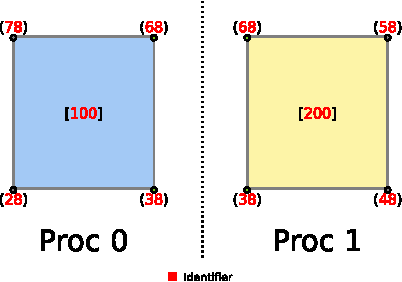
\includegraphics{figures/stkMeshUniversalPart.pdf}
\caption{Parallel-decomposed mesh. Two elements, one on each MPI processor.
Note that some mesh nodes appear on both processors.}
\label{decomp1}
\end{figure}

\begin{figure}[ht]
\centering
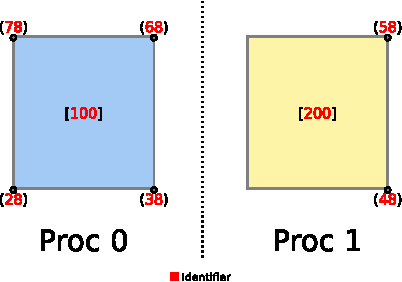
\includegraphics{figures/stkMeshLocallyOwnedPart.pdf}
\caption{Locally-owned nodes.  Nodes 38 and 68 are owned by process 0 and are 
shared but not owned by process 1.}
\label{locallyowned}
\end{figure}

Nalu uses Tpetra::Map objects to identify the degrees of freedom and processor layout.
There are two maps, \code{ownedRowsMap\_} and \code{sharedNotOwnedRowsMap\_}.
For the simple two-element mesh in this example, figure \ref{maps1}
shows how the owned and shared maps would be defined.

\begin{figure}[ht]
\centering
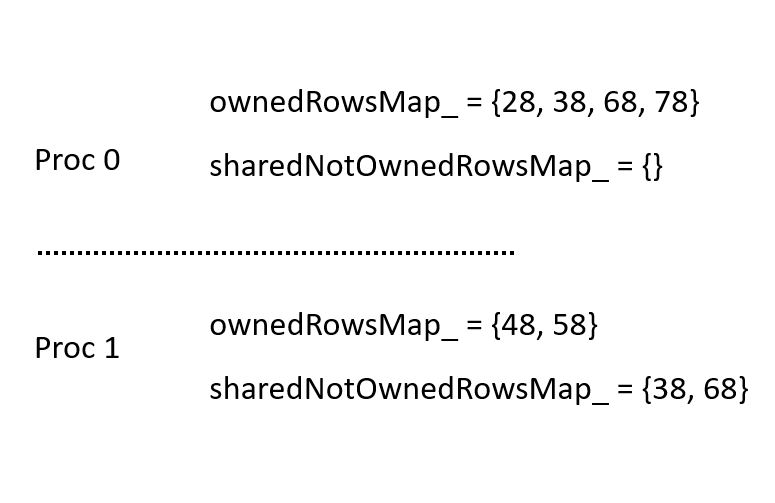
\includegraphics[scale=0.7]{figures/maps1.jpg}
\caption{Owned and Shared-not-Owned Maps.}
\label{maps1}
\end{figure}

We then create \code{Tpetra::CrsGraph} objects for owned and shared
(these objects are called
\code{ownedGraph\_} and \code{sharedNotOwnedGraph\_}), each using the appropriate
row-map. These graphs both use the same column map, and the creation and
initialization of the column map will be discussed in a later section.
We also create Tpetra::CrsMatrix objects for owned and shared, called
\code{ownedMatrix\_} and \code{sharedNotOwnedMatrix\_}.

Each processor contributes an element-matrix of coefficients for its local
elements as shown in figure \ref{elemContribs1}.

\begin{figure}[ht]
\centering
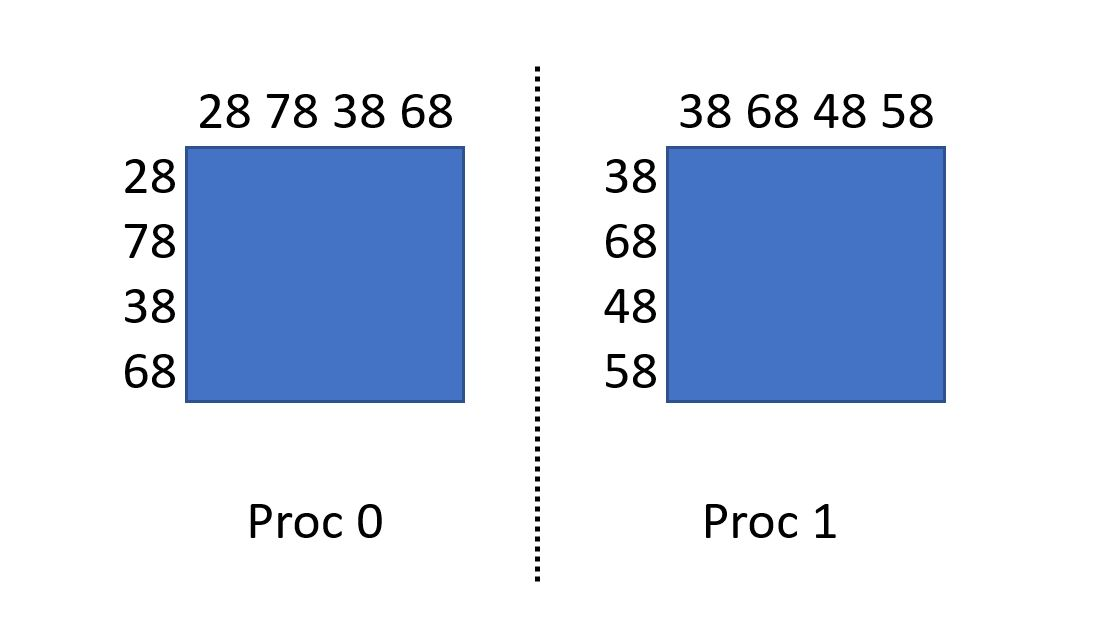
\includegraphics[scale=0.5]{figures/elemContribs.jpg}
\caption{Element-matrix contributions per processor.}
\label{elemContribs1}
\end{figure}

Note that processor 1 has contributions for some rows (38 and 68) that it doesn't
own. Each processor contributes the rows of its element-contributions to
the appropriate matrix object depending on whether the row is owned or not.
Once all element-contributions have been assembled, the contents of the
shared-but-not-owned matrix are sent to the appropriate processors and added
to the owned matrix.
\begin{lstlisting}[caption={Assembly using export}, label=doexport]
  sharedNotOwnedMatrix_->fillComplete();

  ownedMatrix_->doExport(*sharedNotOwnedMatrix_,
                         *exporter_, Tpetra::ADD);

  ownedMatrix_->fillComplete();
\end{lstlisting}
This is done using Tpetra methods as shown in
listing \ref{doexport}. The result is an assembled global matrix as shown
in figure \ref{assembled}.

\begin{figure}[ht]
\centering
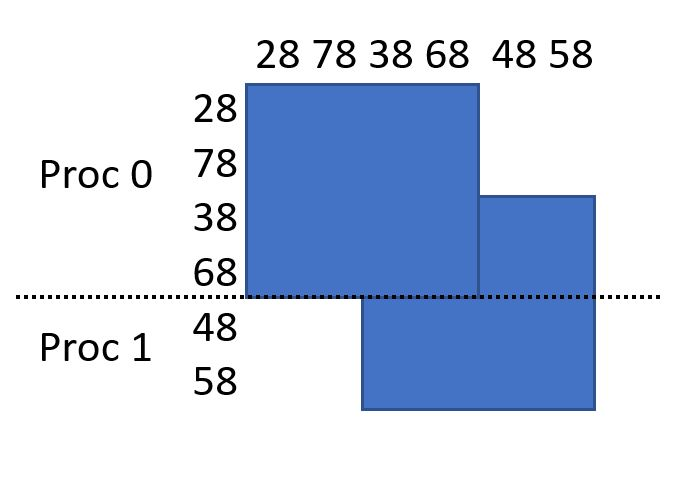
\includegraphics[scale=0.5]{figures/assembled.jpg}
\caption{Assembled \code{ownedMatrix\_}.}
\label{assembled}
\end{figure}

Note that corresponding operations are performed in the assembly of the
right-hand-side vector, in terms of owned and shared, export, etc.

Once the \code{fillComplete} operation has completed, the linear system is
fully assembled and is ready to be passed to solvers and/or preconditioners.
Later sections will go into more detail on the construction of the
column map and graph objects, in order to correctly and efficiently
incorporate off-processor column entries, etc.

We broadly split the construction of the linear system into two
phases called initialization and assembly. The initialization phase
is where we construct the maps, perform communication to send column
indices to appropriate processors, and construct graph objects.
The assembly phase is where we assemble coefficient values into the
matrix using a ``sum-into'' operation, and also modify the linear
system to enforce boundary conditions. In simulations where the structure
of the linear system doesn't change from one timestep to the next, we
can gain efficiency by performing the initialization phase once and
then reusing the data structures for many assembly and solve phases.

Mesh nodes can also be ghosted, which means they are copied from the owning
processor to another processor which has no connectivity relationship with
those nodes. Ghosted nodes (on the receiving processor) are neither owned
nor shared. Ghosting can happen when periodic boundaries of the mesh are mapped
to each other across MPI processors. Ghosting can also happen when a mesh
surface is in contact with another mesh surface where the elements on either
side of the contact don't share connected nodes. See figure \ref{slidingmesh1}
for an example of a mesh with contact boundaries going through the middle. In
this case elements along the sliding boundary can be ghosted to the processor
on the other side of the boundary. When elements are ghosted, the connected nodes
of those elements are also ghosted.

\begin{figure}[ht]
\centering
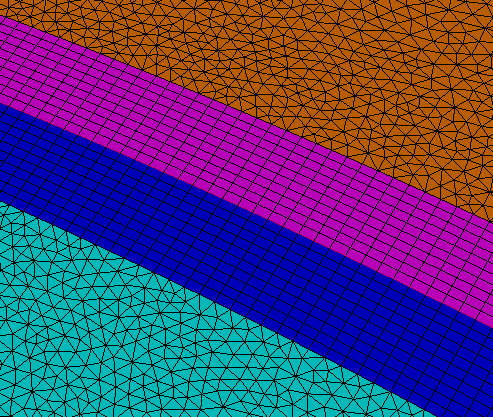
\includegraphics{figures/slidingMesh1.png}
\caption{Mesh with sliding contact boundary.}
\label{slidingmesh1}
\end{figure}

Ghosted nodes don't directly produce equations (rows) in the assembled linear system,
but can result in additional column-entries in other rows.


%&LaTeX

\chapter{Initialization}
Each linear system assembly includes an initialization phase, where the
degrees of freedom and decomposition are defined using Tpetra::Map, and
connectivities are mapped to a compressed row storage (CRS) graph structure.
The following list describes, with some pseudo-code, the broad sequence used
to create and initialize the Tpetra objects. The code that implements these
steps resides in the Nalu class \code{TpetraLinearSystem}.

\begin{enumerate}
\item Create owned and shared maps, and exporter to communicate between them.
\begin{verbatim}
  ownedRowsMap_ = new Map(ownedGlobalIds, ...);
  sharedNotOwnedRowsMap_ = new Map(sharedNotOwnedGlobalIds, ...);
  exporter_ = new Exporter(sharedNotOwnedRowsMap_,
                           ownedRowsMap_);
\end{verbatim}

\item
  Accumulate lists of connectivities defined by
  element-node connections, etc. Currently these connectivity lists are stored
  in a simple vector-of-vectors structure to represent the 'ragged table' of
  node-to-node connections.

\item
  Using mesh information, determine row-lengths due to local connections and due
  to contributions from neighbor processors (which share rows that we own, and
  will thus contribute column-indices to some of our rows). The STK mesh structure
  can tell us the list of neighboring MPI processors, i.e., the MPI processors
  which have portions of the mesh which connect to the local MPI processor's
  portion of the mesh.

  We then traverse our connectivities and for each shared-but-not-owned entity
  we send column entries to the graph on the MPI processor that owns the
  entity. This enables us to compute exact row-lengths for each row in the
  graph.

  Note that this step, and the remaining initialization steps, are implemented
  in the Nalu method \code{TpetraLinearSystem::finalizeLinearSystem()}.

\item
  Create and fill Kokkos::Views representing the local portion of the
  compressed-sparse-row graphs. These are the \code{rowPointers}
  and \code{columnIndices} arrays that will be passed into the
  \code{Tpetra::CrsGraph::setAllIndices} method later. As an implementation
  detail, during construction we hold these Kokkos::Views in a Nalu structure
  called \code{LocalGraphArrays} and this object has methods for inserting
  entries, etc.

\item Construct column map.
  Fill a list of ids representing the union of all column-entries 
  that will be on the local processor. These ids are ordered as
  follows.
\begin{enumerate}
  \item Owned: indices that the local processor owns.
  \item Shared: indices that the local processor shares but doesn't own.
  \item Remote: sometimes called 'reachable', these are indices that
     are neither owned nor shared, but are connected to shared on
     a neighboring processor. These indices are grouped by which
     processor they come from.
\end{enumerate}

\begin{verbatim}
  totalColsMap_ = new Map(colGlobalIds, ...);
\end{verbatim}

\item Construct Graphs.
\begin{verbatim}
  sharedNotOwnedGraph_ = new Graph(sharedNotOwnedRowsMap_,
                                   totalColsMap_, ...);
  ownedGraph_ = new Graph(ownedRowsMap_,
                          totalColsMap_, ...);

  ownedGraph_->setAllIndices(/* our computed local
                                owned-graph indices */);
  sharedNotOwnedGraph_->setAllIndices(/* our computed local
                                         shared-graph indices */);

  importer = new Import(ownedRowsMap_, non-owned-col-ids, source-pids);

  ownedGraph_->expertStaticFillComplete(ownedRowsMap_,
                            ownedRowsMap_, importer, ...);
  sharedNotOwnedGraph_->expertStaticFillComplete(ownedRowsMap_,
                                     ownedRowsMap_, importer, ...);
\end{verbatim}

\item Construct Matrices
\begin{verbatim}
  ownedMatrix_ = new Matrix(ownedGraph_);
  sharedNotOwnedMatrix_ = new Matrix(sharedNotOwnedGraph_);
\end{verbatim}
\end{enumerate}


%&LaTeX

\chapter{Assembly}
The linear system assembly phase is where matrix and rhs-vector contributions
are added, using sum-into APIs.

Nalu computes matrix and rhs-vector contributions in classes which are derived
from the \code{Kernel} base-class. These kernels include computations such as
continuity-advection, momentum-advection-diffusion, and many others. These kernels
are called within an algorithm which manages mesh traversal, handles the gathering
of field-data and master-element computations, etc. The following pseudo-code shows
the execution or flow of these algorithms.

\begin{verbatim}
select buckets for part(s) that algorithm is applied to

for each selected bucket {
   ScratchViews scratch(gathered fields);

   for each elem in bucket {
        fill_scratch_views(scratch, ...);

        for each active kernel {
           kernel->execute(lhs, rhs, scratch);
        }
        sum_into_linear_system(lhs, rhs);
    }
}
\end{verbatim}

Note that in the above pseudo-code, \code{fill\_scratch\_views} includes both
gathering needed field-data as well as making master-element calls such
as grad-op, etc.

Note also that significant detail has been omitted, such as the handling of
SIMD sub-looping, interleaving the SIMD data, etc.  To see the actual algorithm code,
see the Nalu classes \code{AssembleElemSolverAlgorithm},
and \code{AssembleFaceElemSolverAlgorithm}.

The \code{sum\_into\_linear\_system} step is where the computed coefficients are
contributed to the linear-system. This is done by obtaining the local matrix from the
\code{Tpetra::CrsMatrix} object using the method \code{getLocalMatrix()} and then
summing directly into that. Similarly, rhs coefficients are summed into the \code{Kokkos::View}
provided by the \code{getLocalView} method of \code{Tpetra::Vector}.

Recall that we are operating on two matrix objects, \code{ownedMatrix\_} and
\code{sharedNotOwnedMatrix\_}. During this sum-into process, coefficients are added
to the appropriate matrix (and rhs-vector) depending on whether they are associated
with an owned or shared mesh node. Once all local assembly is complete, the shared matrix
is then communicated and added to the local matrix using \code{Tpetra} operations, called
from within the Nalu method \code{TpetraLinearSystem::loadComplete()}:

\begin{verbatim}
sharedNotOwnedMatrix_->fillComplete();

ownedMatrix_->doExport(*sharedNotOwnedMatrix_, *exporter, Tpetra::ADD);

ownedMatrix_->fillComplete();

ownedRhs_->doExport(*sharedNotOwnedRhs_, *exporter_, Tpetra::ADD);
\end{verbatim}

\section{Boundary condition enforcement}

Dirichlet boundary conditions are enforced by modifying the appropriate rows
of the assemled linear system before calling the linear-solver.

Insert pseudo-code for dirichlet BC enforcement here.



\include{index}
\refstepcounter{chapter}
\addcontentsline{toc}{chapter}{Index}
\begin{raggedright}
\begin{footnotesize}
\printindex
\end{footnotesize}
\end{raggedright}
%\include{endmatter}

%
% Comment out distribution list for drafts. 
%
\begin{SANDdistribution}[NM]% or [CA]
  % \SANDdistCRADA	% If this report is about CRADA work
  % \SANDdistPatent	% If this report has a Patent Caution or Patent Interest
  % \SANDdistLDRD	% If this report is about LDRD work

  % External Address Format: {num copies}{Address}
  % \SANDdistExternal{1}{}
  % \bigskip

  % The following MUST BE between the external and internal distributions!
  % \SANDdistClassified % If this report is classified

  % Internal Address Format: {num copies}{Mail stop}{Name}{Org}

  % Mail Channel Address Format: {num copies}{Mail Channel}{Name}{Org}
  %\SANDdistInternalM{}{}{}{}
\end{SANDdistribution}

\end{document}
